% Figure BFS 1
\ffigbox[\FBwidth]{
\caption{\centering Graphe \(G\) privé \\des sommets \(g\) et \(h\)}\label{Fig:td_4_ex_1_2}
}{
    \fbox{
        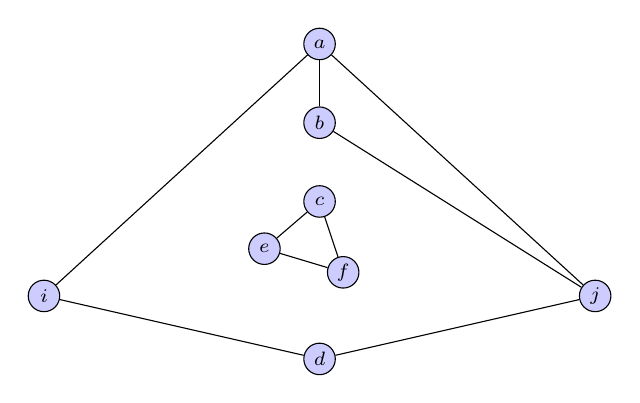
\begin{tikzpicture}[scale=1, every node/.style={circle, draw, fill=blue!20, inner sep=1pt, font=\scriptsize, minimum size=4mm}]
            \node (a) at (0, 2) {\(a\)};
            \node (b) at (0, 1) {\(b\)};
            \node (c) at (0, 0) {\(c\)};
            \node (d) at (0, -2) {\(d\)};

            \node (e) at (-0.7, -0.6) {\(e\)};
            \node (f) at (0.3, -0.9) {\(f\)};

            % \node (g) at (-2, -0.6) {\(g\)};
            % \node (h) at (2, -0.6) {\(h\)};

            \node (i) at (-3.5, -1.2) {\(i\)};
            \node (j) at (3.5, -1.2) {\(j\)};

            \draw (a) -- (b);
            % \draw (a) -- (g);
            \draw (a) -- (i);
            \draw (a) -- (j);

            % \draw (b) -- (g);
            % \draw (b) -- (h);
            \draw (b) -- (j);

            \draw (c) -- (e);
            \draw (c) -- (f);
            % \draw (c) -- (h);

            % \draw (d) -- (g);
            % \draw (d) -- (h);
            \draw (d) -- (i);
            \draw (d) -- (j);

            \draw (e) -- (f);
            % \draw (e) -- (g);

            % \draw (f) -- (h);

            % \draw (g) -- (i);

            % \draw (h) -- (j);
        \end{tikzpicture}
    }
}